%%%%%%%% DO NOT MODIFY %%%%%%%
\documentclass[11pt]{article}
\usepackage{tls}
% \usepackage[italian]{babel}
\usepackage{setspace}
\onehalfspacing

% Any custom packages you wanna use go below this line
% \usepackage{package-name}


% Edit the title, author names and your current email addresses
\title{\liningfont Valutazione degli effetti della sincronizzazione dei semaforie e delle condizioni meteo avverso sul flusso del traffico: simulazione su NetLogo}
\author{\liningfont Beatrice Poli \\ Università degli Studi di Milano-Bicocca \\ \texttt{b.poli1campus.unimib.it}}
\date{}           % Leave date empty

\begin{document}

% DON'T COMMENT/REMOVE THE FOLLOWING 3 LINES
\maketitle
\thispagestyle{empty}
\pagestyle{empty}

% START WRITING YOUR CONTENT BELOW THIS LINE



\section{INTRODUZIONE}
Il traffico automobilistico è una delle maggiori sfide del mondo moderno. Sia in condizioni meteorologiche favorevoli che avverse, la gestione efficiente del traffico può essere difficile da raggiungere. La temporizzazione dei semafori è una delle soluzioni più comuni per migliorare la circolazione del traffico, ma non sempre è facile capire come regolare i tempi per ottenere i migliori risultati.

Il traffico nelle città è infatti molto influenzato dalla quantità di auto che attraversano gli incroci stradali e la velocità con cui le auto passano dipende direttamente dalla temporizzazione dei semafori, ma il tempo meteorologico ha un effetto maggiore in base alla stagione e al clima dell'area in cui ci si trova. Ad esempio, eventi atmosferici come pioggia e neve possono limitare il traffico in alcune aree.

In questo progetto utilizzeremo un modello di agenti basato su NetLogo per analizzare e comprende gli effetti della temporizzazione dei semafori sul flusso traffico dei veicoli in condizioni meteorologiche avverse.

Attraverso l'utilizzo di questo modello, speriamo di ottenere una migliore comprensione delle dinamiche del traffico e di come la temporizzazione dei semafori possa essere ottimizzata per migliorare la circolazione in diverse condizioni climatiche. Questo progetto potrà fornire anche informazioni utili per la pianificazione e la gestione del traffico in generale, ma anche in caso di brutto tempo.

Inizieremo il progetto esaminando la teoria e i concetti fondamentali dei modelli già presenti e della simulazione del traffico. Successivamente, ci concentreremo sulla creazione della simulazione di traffico utilizzando NetLogo e sulla sua configurazione e personalizzazione per soddisfare le nostre esigenze specifiche. Infine, esploreremo i risultati della simulazione e discuteremo le conclusioni e le implicazioni per la gestione del traffico in futuro. Ci sono infatti molte possibilità di estendere e modificare la simulazione come la modellizzazione del flusso di informazioni tra auto controllate dalle persone, auto con guida autonoma e l'infrastruttura di controllo dei semafori.

\section{STATO DELL’ARTE}
Lo stato dell'arte dei modelli di simulazione di traffico stradale si è evoluto negli ultimi anni per tenere conto della crescente complessità del traffico e della necessità di prevedere il suo comportamento. I modelli di simulazione attualmente utilizzati variano da semplici modelli di flusso di traffico basati su equazioni matematiche, a modelli più avanzati che considerano fattori come la congestione, i comportamenti dei conducenti e le restrizioni di capacità.

Gli studi che hanno utilizzato modelli matematici per analizzare il comportamento del traffico, ad esempio, hanno scoperto che la temporizzazione dei semafori ha un impatto significativo sul flusso del traffico e sulla sicurezza stradale.

Inoltre, l'integrazione di tecnologie come l'intelligenza artificiale e l'apprendimento automatico sta portando a modelli di simulazione sempre più sofisticati che possono utilizzare dati in tempo reale e analizzare le tendenze del traffico per prevedere le condizioni future.

Altri studi basati sugli agent based model hanno infatti utilizzato tecniche di intelligenza artificiale per simulare le interazioni tra i veicoli e i semafori e comprendere come la temporizzazione influisca sul traffico.

In generale, i modelli di simulazione di traffico stradale possono essere classificati in tre categorie principali: modelli deterministici, stocastici e basati su agenti.

\subsection{Modelli deterministici}
I modelli deterministici di simulazione di traffico stradale sono modelli matematici che utilizzano equazioni deterministiche per simulare il comportamento del traffico su una rete stradale. Questi modelli cercano di descrivere le interazioni tra i veicoli e il sistema stradale in modo preciso e prevedibile.

Di solito si basano su equazioni che descrivono la dinamica del traffico, ad esempio la distanza tra i veicoli, la velocità e la capacità della strada. Queste equazioni sono risolte numericamente per produrre una simulazione dettagliata del comportamento del traffico.

I modelli deterministici di simulazione di traffico stradale sono molto utili per comprendere le dinamiche del traffico e per prevedere come esso si comporterà in futuro in risposta a determinate condizioni.

Tra questi troviamo il modello di flusso di traffico sviluppato da Kai Nagel e Michael Schreckenberg nel 1992. Questo modello deterministico descrive il comportamento del traffico su una singola corsia in base alle interazioni tra i veicoli. È stato utilizzato con successo per studiare le dinamiche del traffico e ha fornito una comprensione più profonda delle cause della sua congestione e di altri problemi di circolazione.

\subsection{Modelli stocastici}
I modelli stocastici di simulazione di traffico stradale sono modelli che utilizzano processi stocastici per simulare il comportamento del traffico e tengono conto delle incertezze e delle variabili casuali presenti nel traffico reale. Questi modelli sono molto utili per la simulazione di situazioni di traffico complesse, ma possono essere più difficili da implementare e analizzare rispetto ai modelli deterministici, poiché richiedono una comprensione approfondita dei processi stocastici e delle tecniche di simulazione.

Tra i più importanti è presente il modello di sistemi di Markov, il quale è un tipo di modello matematico che utilizza proprio la teoria dei sistemi di Markov per descrivere il comportamento di un sistema dinamico che evolve nel tempo. Il modello suppone che il futuro stato del sistema dipenda solo dallo stato attuale e non dalla sua storia passata.

In un sistema di Markov, gli stati sono descritti da una serie di variabili che cambiano nel tempo e il passaggio da uno stato all'altro è descritto da una probabilità che dipende solo dallo stato attuale. Questo modello è molto utile per la simulazione di sistemi dinamici in cui le incertezze e le variabili casuali sono presenti, come ad esempio il traffico stradale, la diffusione delle malattie e la dinamica dei prezzi dei beni. Ad esempio, in un modello di traffico stradale, la posizione di un veicolo può essere descritta come un processo stocastico che evolve nel tempo in base a una serie di eventi casuali.

\subsection{Modelli basati su agenti}
I modelli di simulazione di traffico stradale basati su agenti sono un tipo di modello di simulazione che utilizza la programmazione basata su agenti per descrivere il comportamento del traffico.

Questi modelli utilizzano una prospettiva decentralizzata per descrivere il comportamento del traffico, in cui ogni agente è visto come un individuo che prende decisioni autonome in base a informazioni locali e a regole predefinite. Questo tipo di modello è molto utile per la simulazione di situazioni complesse in cui il comportamento di un singolo veicolo è influenzato dal comportamento degli altri veicoli e dall'ambiente circostante.

In un modello di traffico stradale basato su agenti, ogni veicolo è descritto da un insieme di attributi, come la posizione, la velocità e le preferenze di guida. Gli agenti possono interagire tra loro e con l'ambiente attraverso un insieme di regole predefinite che descrivono come ogni agente dovrebbe comportarsi in determinate situazioni.

I modelli di simulazione di traffico stradale basati su agenti sono molto utili per la simulazione di situazioni complesse, poiché descrivono il comportamento del traffico in un modo che tiene conto della complessità delle interazioni tra veicoli e ambiente. Questo tipo di modello è spesso utilizzato per studiare gli effetti di vari fattori, come la temporizzazione dei semafori, la presenza di incidenti o condizioni meteorologiche avverse sul traffico.

In generale, i modelli di simulazione di traffico sono composti da una componente di modellizzazione che descrive il suo comportamento, una componente di input che fornisce i dati sulla rete stradale e le condizioni iniziali, e una componente di output che presenta i risultati della simulazione. La scelta del modello di simulazione più appropriato dipende dalla complessità del problema e dagli obiettivi specifici della simulazione.

Tuttavia, ci sono ancora sfide nello sviluppo di modelli di simulazione di traffico affidabili e precisi, inoltre, la complessità del comportamento del traffico e la sua dipendenza dalle condizioni ambientali e sociali rendono difficile prevedere con precisione il suo comportamento futuro.

Infatti, la maggior parte di questi studi si concentra sul traffico in condizioni meteorologiche favorevoli e poco è stato fatto per analizzare gli effetti della temporizzazione dei semafori sul traffico in condizioni meteorologiche avverse.

\section{DESCRIZIONE DEL MODELLO}
Il modello di Nagel-Schreckenberg (NaSch) descrive il traffico come una serie di veicoli che si muovono lungo una corsia in una direzione. Ogni veicolo è descritto da una posizione e una velocità, e i veicoli interagiscono tra loro in base a un insieme di regole.

Esso è dunque un modello di simulazione del traffico automobilistico su una strada a senso unico, che utilizza un approccio computazionale basato su regole e condizioni predefinite.
Il modello considera ogni veicolo come un'entità discreta che si muove ad una velocità costante $v$ e che può subire una frenata per evitare collisioni con i veicoli che la precedono. Ogni veicolo ha una lunghezza $L$, e la distanza tra due veicoli consecutivi è indicata con $d$. 

Le regole di base del modello includono:
\begin{itemize}
\item \underline{Accelerazione:} ogni veicolo accelera a una velocità $v$ fino a raggiungere la velocità massima consentita $v_\max$, a meno che non ci sia un veicolo più lento davanti a lui che si trova ad una distanza $d<v$.

\item \underline{Frenata:} se la distanza $d$ tra due veicoli consecutivi è inferiore alla velocità $v$ del veicolo che segue, il veicolo che segue deve frenare a una velocità uguale a $d-I$.

\item \underline{Casualità:} per evitare che i veicoli si muovano tutti alla stessa velocità, viene introdotta una componente casuale nell'accelerazione dei veicoli.

\item \underline{Movimento:} una volta che un veicolo ha accelerato o frenato, si sposta avanti di una distanza pari alla sua velocità.
\end{itemize}

\begin{figure}
    \centering
    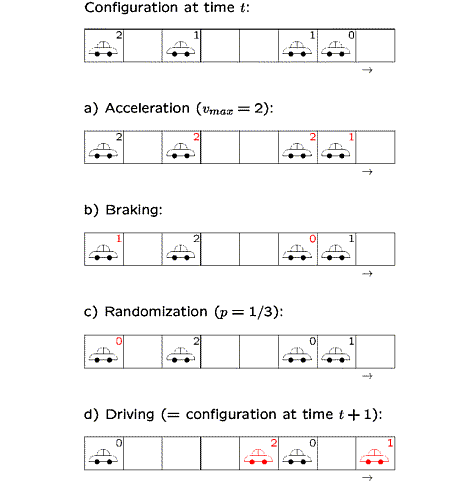
\includegraphics[width=0.6\textwidth]{trafficflow.png}
    \caption{Modello di Nagel-Schreckenberg}
    % \label{fig:my_label}
\end{figure}

La prima regola rappresenta l'aumento graduale della velocità dei veicoli, uno spazio alla volta, in base allo spazio disponibile. La seconda regola impone la decelerazione o l'arresto in caso di presenza di un veicolo precedente. Questa regola ha due implicazioni: è asimmetrica rispetto all'accelerazione, il che significa che un veicolo può decelerare molto più velocemente di quanto acceleri, e rende impossibili le collisioni. La terza regola simula la decelerazione casuale e spontanea dell'automobilista, che è di fondamentale importanza per evitare che il modello sia completamente deterministico. Infine, la quarta regola determina l'avanzamento dei veicoli in base alle regole precedenti. Nonostante il modello utilizzi delle semplificazioni a livello microscopico, le conseguenze a livello macroscopico sono estremamente positive. La dimostrazione di ciò è data dalla capacità del modello di replicare in modo efficace il traffico reale, che è rappresentato dalla relazione tra il flusso di veicoli (ovvero il numero di veicoli che passa in una determinata unità di tempo) e la densità (ovvero il numero di veicoli presenti in un determinato spazio).

Il modello tiene conto anche dell'effetto di "onda di congestione", che si verifica quando una frenata improvvisa da parte di un veicolo provoca una reazione a catena che si propaga all'indietro nella fila di veicoli. La posizione di ogni veicolo viene dunque aggiornata in base alla sua velocità.

Il modello di Nagel-Schreckenberg è stato utilizzato con successo per studiare le dinamiche del traffico, come la formazione di ingorghi e la transizione tra flusso libero e congestione.

Il suddetto modello ha ispirato lo sviluppo di numerosi altri modelli di simulazione del traffico, sia in ambito accademico che industriale. Ad esempio, il modello è stato utilizzato come punto di partenza per la creazione di varianti che prendono in considerazione fattori come la presenza di veicoli pesanti e l'effetto degli incidenti stradali.

Tra i modelli che si sono ispirati a quello di Nagel e Schreckenberg c'è sicuramente l'Intelligent driver model (IDM), che spiegheremo di seguito.

\textbf{Treiber, Hennecke and Helbing (2000)} - L'Intelligent Driver Model (IDM) è un modello di traffico per la simulazione di autostrade e strade urbane che descrive il comportamento dei conducenti nell'accelerazione, nella decelerazione e nella distanza di sicurezza tra i veicoli.

Il modello IDM si basa su alcune assunzioni fondamentali, tra cui: ogni veicolo si comporta come un agente razionale che cerca di mantenere una distanza di sicurezza dalla vettura antecedente e di raggiungere una velocità obiettivo in modo efficiente, evitando le collisioni. 

In dettaglio, il modello IDM, come il modello $\mathrm{NaSch}$, tiene conto di quattro fattori principali:
\begin{itemize}
\item \underline{Accelerazione:} la velocità a cui un veicolo accelera dipende dalla differenza tra la velocità attuale e la velocità obiettivo, la distanza di sicurezza e la decelerazione massima.

\item \underline{Decelerazione:} un veicolo può decelerare in modo graduale o brusco, a seconda della distanza di sicurezza, della differenza di velocità e dell'accelerazione massima.

\item \underline{Distanza di sicurezza:} la distanza tra un veicolo e il veicolo antecedente dipende dalla velocità relativa, dalla velocità attuale e dalla velocità obiettivo, nonché da una costante di sicurezza.

\item \underline{Velocità obiettivo:} la velocità a cui un veicolo tende a raggiungere, in funzione delle condizioni del traffico e delle limitazioni della strada.
\end{itemize}


\section{ESTENSIONE DEL MODELLO}
Il paragrafo "estensione del modello" spiega che i modelli di simulazione del traffico come quello di Nagel e Schreckenberg, pur essendo molto precisi nella descrizione del comportamento dei singoli veicoli, non tengono conto di molte altre variabili che possono influire sul traffico in una rete stradale. Ad esempio, le condizioni meteorologiche avverse possono influenzare la visibilità e la tenuta del manto stradale, mentre la presenza di semafori può causare ingorghi e rallentamenti del traffico.

Per ovviare a queste limitazioni, è stato sviluppato un modello di rete stradale che tiene conto di queste variabili aggiuntive, fornendo una rappresentazione più precisa e completa del traffico su una rete stradale. Questo modello più avanzato prevede l'inserimento di condizioni meteorologiche avverse e la presenza di semafori temporizzati.

Questo tipo di modello di simulazione è utile per la pianificazione del traffico, la progettazione di infrastrutture stradali e la valutazione delle politiche di mobilità sostenibile.

Infatti, consente di valutare gli effetti di diverse variabili sulla circolazione stradale, come la densità del traffico, la velocità media e i tempi di percorrenza, e può aiutare a prevedere l'impatto di interventi strutturali e organizzativi sulla mobilità urbana ed extraurbana.

\subsection{Il modello su Netlogo}
È stato creato un modello di simulazione del traffico utilizzando Netlogo, un software di simulazione basato su agenti il quale risulta essere adatto per la simulazione di sistemi complessi e distribuiti come il traffico stradale.

La scelta di utilizzare Netlogo è stata fatta in quanto offre un ambiente di programmazione semplice e una vasta libreria di componenti che possono essere utilizzati per la creazione di modelli di traffico. Questo modello di simulazione è un metodo efficace che può essere utilizzato su un sistema reale già esistente, in modo da riuscire a studiare quali saranno $\mathrm{i}$ risultati rendendo così possibili delle modifiche, o per progettare un nuovo sistema

La simulazione prevede un ambiente composto da due strade che si incrociano con una corsia per ogni direzione. Il traffico è regolato da semafori che cambiano in base a un determinato programma. I veicoli sono rappresentati come agenti che seguono il semaforo e si muovono lungo le strade per raggiungere la loro destinazione. Ogni auto è modellata utilizzando un approccio basato sull'agente che tiene conto dei loro meccanismi decisionali e delle interazioni con altre auto nell'ambiente.

Il modello è stato utilizzato per esplorare la dinamica del traffico e il flusso di veicoli all'intersezione, con l'obiettivo di comprendere come le variabili come il numero di veicoli e la velocità dei veicoli influiscono sul traffico e sul tempo di percorrenza.

\begin{figure}
    \centering
    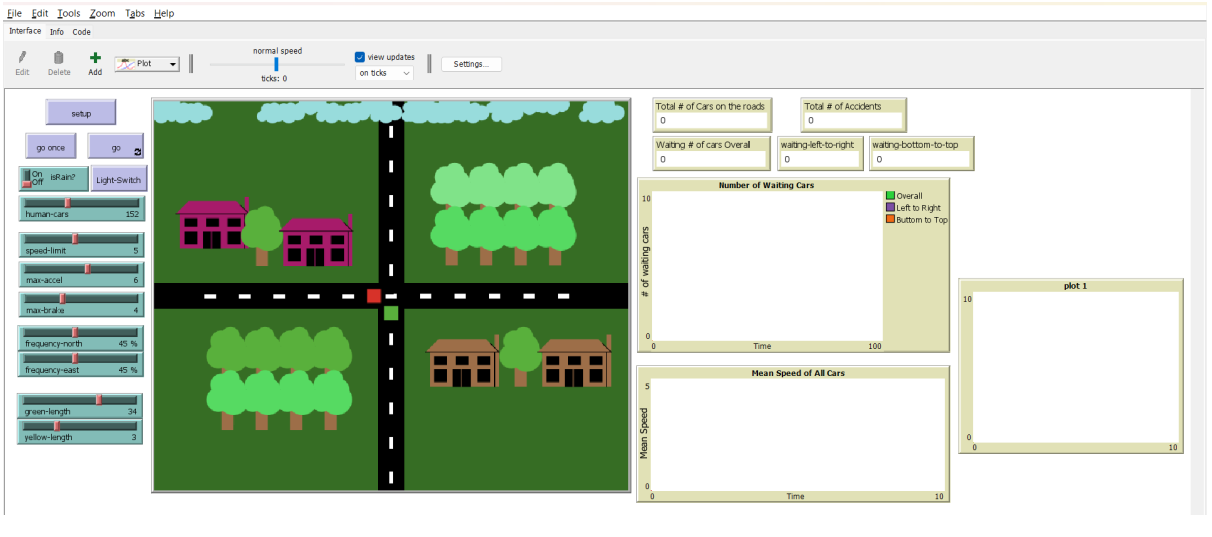
\includegraphics[width=1\textwidth]{fig1.png}
    \caption{Modello di simulazione svilupatto su Netlogo}
    % \label{fig:my_label}
\end{figure}


\subsection{Parametri}
\begin{itemize}
\item Per impostare o reimpostare la simulazione, premere setup
\item Per far muovere le auto una volta, premere \textit{go once}
\item Per far muovere le auto all'infinito, premere \textit{go}
\item Premere nuovamente il pulsante go per fermare le automobili.
\item \textit{Rain} switch - spostare la levetta per far piovere o meno
\item \textit{car}-\textit{number} - determina il numero di macchine guidate da persone all'interno della rete stradale
\item \textit{speed}-\textit{limit} slider - determina il limite di velocità della città
\item \textit{max}-\textit{accel} slider - impostare la velocità fino a cui le automobili possono accelerare
\item \textit{max}-\textit{brake} slider - impostano la velocità con cui le macchine frenano
\item \textit{frequency}-\textit{north} slider - seleziona la frequenza con cui le nuove automobili dirette a nord si spostano sulla strada
\item \textit{frequency}-\textit{east} slider - seleziona la frequenza con cui le nuove auto dell'est guidano su strada
\item \textit{num}-\textit{of}-\textit{cars} - determina quante auto ci sono nella rete stradale
\item \textit{lights}-\textit{interval} - determina il tempo tra i semafori
\item \textit{waiting}-\textit{time}-\textit{overall} - visualizza il numero totale di auto in attesa durante uno specifico ticchettio dell'orologio
\item \textit{waiting}-\textit{left}-\textit{to}-\textit{right} - visualizza il numero di automobili dirette a est in attesa in un dato momento
\item \textit{waiting}-\textit{bottom}-\textit{to}-\textit{top} - visualizza il numero di automobili dirette a nord in attesa in un dato momento
\end{itemize}


\section{SIMULAZIONE}
Dopo che tutti i comportamenti descritti sopra sono stati implementati in Netlogo, il passo successivo è stato eseguire alcune simulazioni del modello e verificare se il comportamento dei veicoli corrispondesse alle aspettative prefissate in corrispondenza del modello originale. 

Nel modello di simulazione basato su agenti, sono stati testati circa 20 scenari diversi per analizzare l'impatto del tempo di segnalazione del semaforo sul flusso del traffico e sulla congestione del traffico in condizioni climatiche avverse. L'obiettivo era di comprendere come le tempistiche del semaforo potessero influire sulla congestione del traffico e come le condizioni atmosferiche potessero a loro volta influire su quest'ultimo.

Sono state provate le seguenti combinazioni:

\underline{SENZA PIOGGIA:}

\begin{tabular}{c l l}
$\bullet$ & \textbf{max-accel:} 2 & \textbf{max-brake:} 7\\
$\bullet$ & \textbf{max-accel:} 8 & \textbf{max-brake:} 3\\
&& \\
$\bullet$ & \textbf{green-lenght:} 40 & \textbf{yellow-lenght:} 2\\
$\bullet$ & \textbf{green-lenght:} 45 & \textbf{yellow-lenght:} 3
\end{tabular}


\underline{CON PIOGGIA:}

\begin{tabular}{c l l}
$\bullet$ & \textbf{max-accel:} 2 & \textbf{max-brake:} 7\\
$\bullet$ & \textbf{max-accel:} 8 & \textbf{max-brake:} 3\\
&& \\
$\bullet$ & \textbf{green-lenght:} 40 & \textbf{yellow-lenght:} 2\\
$\bullet$ & \textbf{green-lenght:} 45 & \textbf{yellow-lenght:} 3
\end{tabular}

\section{ANALISI}
La simulazione del traffico è un campo di ricerca in costante evoluzione. Un modello di simulazione del traffico come quello di Nagel e Schreckenberg è utile per comprendere il comportamento dei veicoli individuali all'interno di una rete stradale, tuttavia ha dei limiti in quanto non tiene conto di molte variabili che possono influire sul traffico, come le condizioni meteorologiche avverse o la presenza di semafori.

Per superare questi limiti, è stato sviluppato un modello di rete stradale utilizzando il software di simulazione NetLogo. Rispetto al modello iniziale sono stati aggiunti dei semafori temporizzati e la pioggia, in modo da rappresentare più fedelmente la realtà.

Dopo aver eseguito la simulazione in diverse condizioni, sono stati confrontati i risultati con quelli del modello di Nagel e Schreckenberg.

I risultati del modello mostrano che il tempo di segnalazione del semaforo ha un impatto significativo sul flusso del traffico in condizioni climatiche avverse. Ad esempio, si nota che un aumento del tempo di segnalazione del semaforo può migliorare la capacità del sistema stradale di gestire il traffico durante le tempeste, ma può anche causare una congestione durante le condizioni climatiche più moderate.

Dai risultati ottenuti dalla simulazione basata su agenti effettuata utilizzando il modello NetLogo, si evidenzia che la variazione del tempo di segnalazione del semaforo giallo ha un impatto significativo sulla congestione del traffico. In particolare, una riduzione del tempo di segnalazione del semaforo giallo si traduce in un aumento della congestione del traffico, mentre un aumento del tempo di segnalazione del semaforo giallo porta ad una diminuzione dell traffico. Questi risultati suggeriscono che una tempistica ottimale del semaforo può avere un effetto positivo sul flusso e sulla congestione del traffico.

Inoltre, i risultati hanno dimostrato che anche la variazione del tempo di frenata ha un impatto significativo sul flusso e sulla congestione del traffico. In particolare, una riduzione del tempo di frenata ha portato ad un aumento degli incidenti sulla rete stradale simulata. Questi risultati sottolineano l'importanza di considerare anche il tempo di frenata nella valutazione delle tempistiche ottimali del semaforo per ottenere un flusso del traffico sicuro e fluido.

Proprio come dimostra il modello NaSch (Nagel-Schreckenberg), i risultati del modello basato su agenti Netlogo hanno confermato che l'aumento del numero di veicoli sulla rete stradale porta ad un aumento della congestione.

Come detto in precedenza, il modello di Nagel e Schreckenberg è un modello di simulazione di traffico stradale che può essere utilizzato per studiare il comportamento del traffico in diverse situazioni, tra cui anche la densità.

In questo modello, la densità del traffico si riferisce al numero di veicoli presenti in una certa area di strada, ad esempio un chilometro. Quando la densità del traffico è bassa, cioè ci sono pochi veicoli sulla strada, i veicoli possono muoversi a velocità relativamente alte e questo creerà poco o nessun ingorgo. Tuttavia, quando la densità del traffico aumenta, cioè ci sono più veicoli sulla strada, la velocità media dei veicoli diminuisce e può verificarsi un ingorgo. 

In generale, il modello di Nagel e Schreckenberg mostra che la densità del traffico ha un impatto significativo sul comportamento del traffico e sulla velocità media dei veicoli. Quando la densità del traffico è molto alta, possono verificarsi fenomeni di congestione e rallentamento del traffico. Questi fenomeni possono essere evitati o ridotti tramite una pianificazione intelligente delle infrastrutture stradali, una gestione efficiente del traffico e una regolamentazione adeguata delle velocità dei veicoli.

Anche il modello sviluppato su NetLogo per simulare il traffico stradale ha confermato l'importanza della densità del traffico sulla sua fluidità e sulla presenza di congestione. In particolare, quando il numero di veicoli aumentava, si verificava un aumento della congestione del traffico. Tuttavia, si è osservato che la densità del traffico diminuiva leggermente quando veniva ottimizzata la regolazione dei semafori.

\begin{figure}
    \centering
    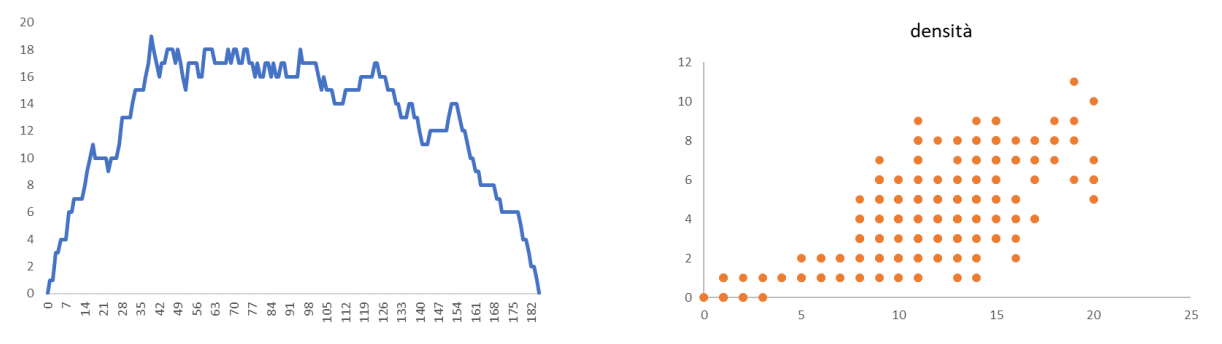
\includegraphics[width=1\textwidth]{fig2.png}
    \caption{Grafici ottenuti dal modello} 
\end{figure}

Questi risultati suggeriscono nuovamente che una pianificazione intelligente delle infrastrutture stradali e una regolamentazione adeguata del traffico possono contribuire a ridurre l'effetto della densità del traffico sulla congestione e sulla fluidità del traffico.

\section{CONCLUSIONI}
In conclusione, la simulazione del traffico è uno strumento molto utile per la progettazione di infrastrutture stradali e la valutazione delle politiche di mobilità sostenibile. L'utilizzo di un modello di rete stradale che tenga conto di molte variabili importanti per il traffico, come le condizioni meteorologiche avverse o la presenza dei semafori, consente di ottenere una rappresentazione più accurata del comportamento del traffico, e quindi di pianificare interventi più efficaci per migliorare la mobilità urbana.

Inoltre, questi risultati possono essere utili per la progettazione di sistemi di controllo del traffico e di regolazione dei semafori più efficienti e per la pianificazione di nuove infrastrutture stradali. In generale, la simulazione del traffico attraverso modelli come quelli di Nagel e Schreckenberg o su NetLogo può fornire importanti informazioni su come migliorare la sicurezza e l'efficienza del traffico stradale.

\subsection{Sviluppi futuri}
Gli sviluppi futuri di un progetto di NetLogo di una simulazione di una rete stradale regolata da semafori che analizza anche l'influenza del meteo avverso potrebbero includere l'estensione del modello per simulare intersezioni multiple oppure integrare una simulazione ibrida dove una parte dei veicoli sono autonomi.
Inoltre, si potrebbe raccogliere dati sul traffico e sulle condizioni meteo reali dalla città in cui viene applicato il modello per migliorare l'accuratezza dei parametri dell'effetto del meteo. Un altro possibile sviluppo futuro potrebbe essere quello di implementare ulteriori variabili ambientali nel modello di simulazione, come ad esempio la presenza di ostacoli, l'aggiunta di corsie per le biciclette o il traffico pedonale. Inoltre, sarebbe possibile utilizzare il modello per simulare scenari di emergenza, come ad esempio eventi naturali, per valutare l'efficacia delle procedure di evacuazione e di gestione del traffico in queste situazioni.
Un'ulteriore prospettiva di sviluppo futuro potrebbe riguardare l'introduzione di algoritmi di intelligenza artificiale per la gestione del traffico. Ad esempio, sarebbe possibile utilizzare algoritmi di apprendimento automatico per prevedere il flusso del traffico in base alle condizioni ambientali e per ottimizzare la sincronizzazione dei semafori in tempo reale.
Infine, sarebbe interessante esplorare l'interazione tra il modello di simulazione del traffico e altri modelli di simulazione, come ad esempio modelli di inquinamento atmosferico o di consumo di carburante. In questo modo sarebbe possibile valutare l'impatto delle politiche di mobilità sostenibile sul traffico e sull'ambiente.


\nocite{*}
\newpage
\bibliography{references}

\end{document}
